\chapter{\textit{Modelagem dinâmica}}

\section{Modelagem do quadrirrotor}
Um quadricóptero é um tipo de veículo aéreo não tripulado(VANT), caracterizado por ter quatro rotores, que podem ser dispostos em diversas configurações. O Parrot Mambo, utilizado nesse trabalho, dispõe de uma configuração em X, sendo que cada rotor pode variar sua velocidade e direção de giro de maneira independente.

Para estudar as características dinâmicas e o sistema de controle do quadrirrotor deste trabalho, é necessário entender como as forças que interagem com o corpo se relacionam. A análise dinâmica de um drone pode ser dividida na dinâmica de corpo rígido, dinâmica translacional, cinemática e dinâmica de atitude, forças agindo sobre o corpo e controle. Neste capítulo, será apresentada essa análise.

\subsection{Configurações do quadricóptero}
O Parrot Mambo é um quadricóptero, consistindo de 4 atuadores (conjunto motor e hélice), que são controlados individualmente para gerar empuxo. Dois dos motores giram no sentido horário e dois no anti-horário para que o momento resultante em torno do centro de massa seja zero, prevenindo movimentos indesejados.

O quadricóptero deste estudo tem uma configuração em 'X', que apresenta desempenho de controle superior em rolagem e arfagem (aproximadamente 30\% de vantagem) em relação à configuração em '+', pois utiliza os 4 motores para esses movimentos (Niemiec e Gandhi, 2014). Independentemente da configuração, o quadricóptero tem 6 graus de liberdade, divididos em três para movimento de translação nos eixos \( X \), \( Y \), \( Z \) e três para movimento de rotação em \( \phi \) (rolagem), \( \theta \) (arfagem) e \( \psi \) (guinada).

No entanto, o quadricóptero é sub-atuado, pois tem apenas 4 atuadores. Isso significa que ele não pode controlar diretamente todos os seus movimentos, como deslocar-se lateralmente sem antes rotacionar na direção desejada. Para superar essa limitação, ele combina rotações e empuxo.

\subsection{Sistemas de coordenadas}
Para a modelagem dinâmica de um quadricóptero, consideramos o sistema de coordenadas inercial $\boldsymbol{\vec{I}}$ = [$\boldsymbol{\vec{X}}$, $\boldsymbol{\vec{Y}}$, $\boldsymbol{\vec{Z}}$], fixo no espaço, e o sistema de coordenadas local $\boldsymbol{\vec{B}}$ = [$\boldsymbol{\vec{X_L}}$, $\boldsymbol{\vec{Y_L}}$, $\boldsymbol{\vec{Z_L}}$], que se move com o quadricóptero.

\begin{figure}[H]
	\centering
	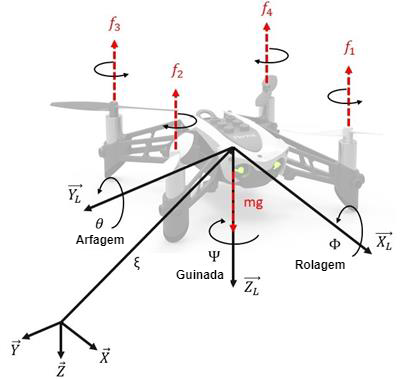
\includegraphics[width=0.6\textwidth]{coordinate-system.png}
	\caption{Representação do sistema de referência inercial e do sistema centralizado no corpo do drone. Fonte: Adaptado de Zaraza Espinosa e Buitrago Galvan (2023).}
	\centering
	\label{fig:coordinate-system}
\end{figure}

\subsection{Matrizes de rotação}
Agora que os sistemas de referência estão definidos, é necessário relacionar o sistema de referência inercial ($\boldsymbol{\vec{I}}$) com o sistema de referência do corpo ($\boldsymbol{\vec{B}}$) por meio da matriz de rotação $R_{bi}$. Essa matriz é obtida através de três rotações sucessivas ao longo dos eixos do sistema inercial (sequência x-y-z), conforme ilustrado a seguir:

\[
	R_{bi}(\phi,\theta,\psi) = R_z(\psi) R_y(\theta) R_x(\phi) =
	\begin{bmatrix}
		cos_\theta cos_\psi & sin_\phi sin_\theta cos_\psi - cos_\phi sin_\psi & cos_\phi sin_\theta cos_\psi + sin_\phi sin_\psi \\
		cos_\theta sin_\psi & sin_\phi sin_\theta sin_\psi + cos_\phi cos_\psi & cos_\phi sin_\theta sin_\psi - sin_\phi cos_\psi \\
		-sin_\theta         & sin_\phi cos_\theta                              & cos_\phi cos_\theta
	\end{bmatrix}
\]

---

\section{Movimentos do Quadricóptero}
Agora que as características do quadricóptero e as suas configurações foram discutidas, vamos descrever os movimentos que ele pode realizar, associados aos seus 6 graus de liberdade. Cada movimento está relacionado a uma combinação de empuxo gerado pelos atuadores e rotações controladas para superar as limitações do sistema sub-atuado.

\subsection{Movimento de Rolagem (Roll - $\phi$)}
A rotação em torno do eixo longitudinal ($X$) do quadricóptero, chamada de rolagem, ocorre quando os motores de um lado geram mais empuxo que os motores do lado oposto, inclinando o quadricóptero lateralmente.

\begin{figure}[H]
	\centering
	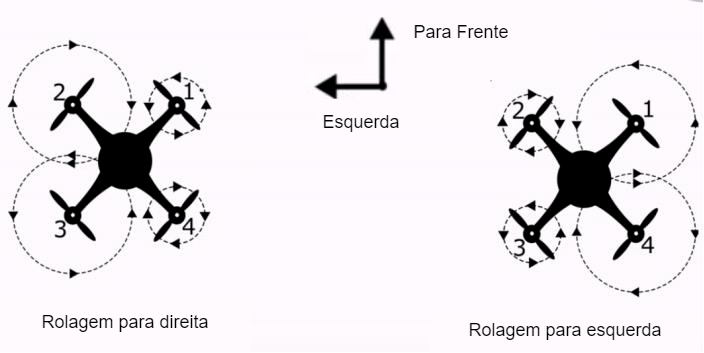
\includegraphics[width=0.8\textwidth]{rolagem-motores.png}
	\caption{Movimento de Rolagem em um quadricóptero com configuração em "X" (Ceppi, 2020).}
	\label{fig:roll_maneuver}
\end{figure}

\begin{figure}[H]
	\centering
	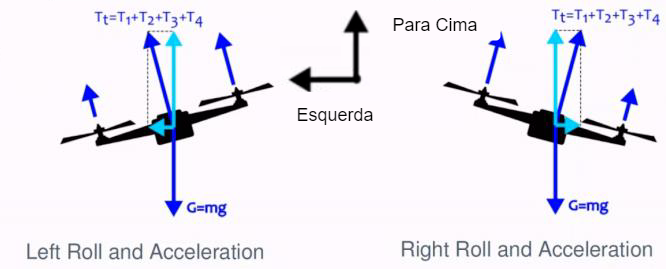
\includegraphics[width=0.8\textwidth]{rolagem-movimento.png} % Substitua por seu caminho de imagem
	\caption{Balanço das forças durante a manobra de Rolagem (Ceppi, 2020).}
	\label{fig:roll_maneuver_forces}
\end{figure}



\subsection{Movimento de Arfagem (Pitch - $\theta$)}
A arfagem corresponde à rotação em torno do eixo lateral ($Y$), inclinando o quadricóptero para frente ou para trás. Esse movimento resulta do diferencial de empuxo entre os motores dianteiros e traseiros.

\begin{figure}[H]
	\centering
	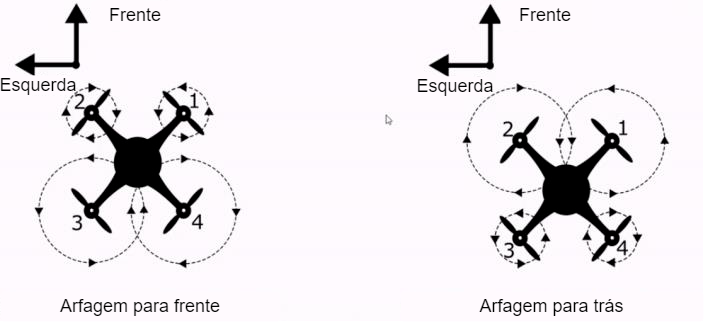
\includegraphics[width=0.8\textwidth]{arfagem-motores.png}
	\caption{Movimento de Arfagem em um quadricóptero com configuração em "X" (Ceppi, 2020).}
	\label{fig:pitch_maneuver}
\end{figure}

\begin{figure}[H]
	\centering
	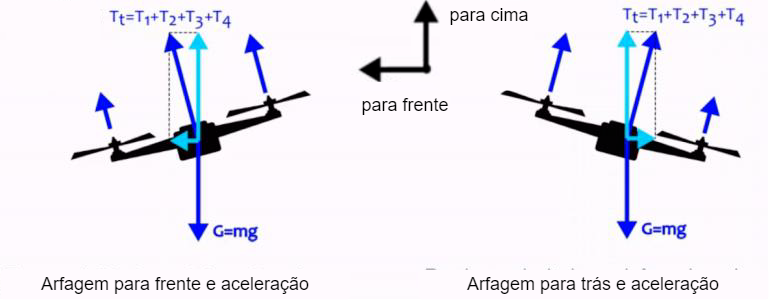
\includegraphics[width=0.8\textwidth]{arfagem-movimento.png} % Substitua por seu caminho de imagem
	\caption{Balanço das forças durante a manobra de Arfagem (Ceppi, 2020).}
	\label{fig:pitch_maneuver_forces}
\end{figure}



\subsection{Movimento de Guinada (Yaw - $\psi$)}
A guinada refere-se à rotação em torno do eixo vertical ($Z$), que altera a direção do quadricóptero. Isso é conseguido ao variar as rotações dos motores no sentido horário e anti-horário, criando um momento resultante que gira o quadricóptero.

\begin{figure}[H]
	\centering
	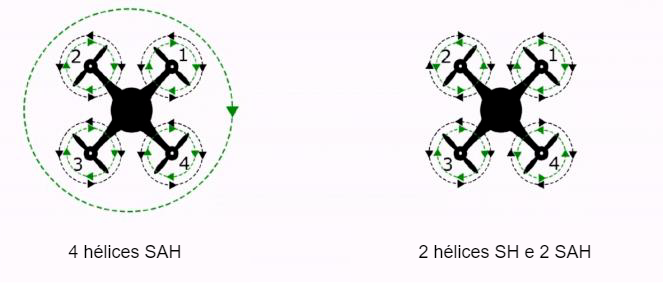
\includegraphics[width=0.8\textwidth]{guinada-motores-movimento.png}
	\caption{Balanço dos torques (Ceppi, 2020).}
	\label{fig:yaw_torques}
\end{figure}


\begin{figure}[H]
	\centering
	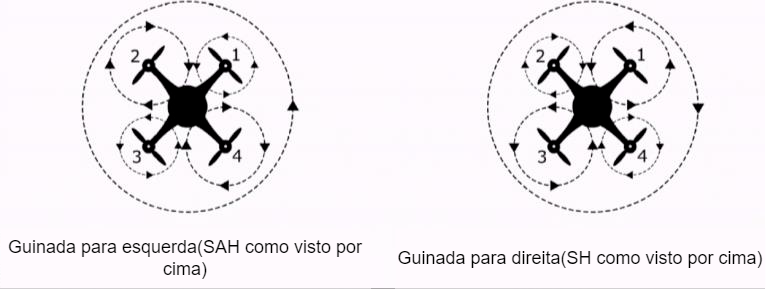
\includegraphics[width=0.8\textwidth]{guinada-movimento.png} % Substitua por seu caminho de imagem
	\caption{Manobra de Guinada e balanço dos torques (Ceppi, 2020).}
	\label{fig:yaw_maneuver_torques}
\end{figure}

\subsection{Forças e Momentos}

A rotação das hélices gerada pelos motores produz forças de sustentação (empuxo) e momentos sobre o quadricóptero. Essas forças e momentos são fundamentais para o controle e a estabilidade do voo. Nesta seção, detalharemos como essas forças e momentos são calculados e como influenciam a dinâmica do quadricóptero.

\subsubsection{Forças Geradas pelas Hélices}

O empuxo produzido por cada hélice é resultado direto da rotação imposta pelo motor. A força de empuxo \( F_i \) gerada pela \( i \)-ésima hélice pode ser expressa pela seguinte equação:

\begin{equation}
F_i = \frac{1}{2} \rho A C_T r_h^2 \Omega_i^2
\label{eq:forca_empuxo}
\end{equation}

Onde:

- \( \rho \) é a densidade do ar (kg/m³).
- \( A \) é a área varrida pela hélice (m²).
- \( C_T \) é o coeficiente de sustentação da hélice (adimensional).
- \( r_h \) é o raio da hélice (m).
- \( \Omega_i \) é a velocidade angular da \( i \)-ésima hélice (rad/s).

Considerando que a densidade do ar e as características geométricas da hélice são constantes durante o voo em baixas altitudes, podemos simplificar a equação definindo uma constante de força \( K_f \):

\begin{equation}
K_f = \frac{1}{2} \rho A C_T r_h^2
\label{eq:constante_forca}
\end{equation}

Assim, a força de empuxo simplifica para:

\begin{equation}
F_i = K_f \Omega_i^2
\label{eq:forca_empuxo_simplificada}
\end{equation}

Essa relação indica que o empuxo é proporcional ao quadrado da velocidade angular da hélice.

\subsubsection{Momentos Gerados pelas Hélices}

Além do empuxo, as hélices geram momentos devido ao torque necessário para mantê-las em rotação. O momento \( M_i \) produzido pela \( i \)-ésima hélice é dado por:

\begin{equation}
M_i = \frac{1}{2} \rho A C_D r_h^2 \Omega_i^2
\label{eq:momento_helice}
\end{equation}

Onde:

- \( C_D \) é o coeficiente de arrasto da hélice (adimensional).

Definimos então uma constante de momento \( K_m \):

\begin{equation}
K_m = \frac{1}{2} \rho A C_D r_h^2
\label{eq:constante_momento}
\end{equation}

O momento produzido pela hélice torna-se:

\begin{equation}
M_i = K_m \Omega_i^2
\label{eq:momento_helice_simplificado}
\end{equation}

\subsubsection{Força Resultante no Quadricóptero}

Considerando que as forças de empuxo atuam ao longo do eixo \( z_b \) do referencial do corpo, a força total atuante no quadricóptero é a soma das forças individuais:

\begin{equation}
\mathbf{F}_b = \begin{bmatrix}
0 \\
0 \\
- \sum_{i=1}^{4} F_i
\end{bmatrix}
= \begin{bmatrix}
0 \\
0 \\
- K_f (\Omega_1^2 + \Omega_2^2 + \Omega_3^2 + \Omega_4^2)
\end{bmatrix}
\label{eq:forca_total_quadricoptero}
\end{equation}

Definindo o empuxo total \( T \):

\begin{equation}
T = K_f (\Omega_1^2 + \Omega_2^2 + \Omega_3^2 + \Omega_4^2)
\label{eq:empuxo_total}
\end{equation}

A força resultante simplifica para:

\begin{equation}
\mathbf{F}_b = \begin{bmatrix}
0 \\
0 \\
- T
\end{bmatrix}
\label{eq:forca_resultante_simplificada}
\end{equation}

Essa é a força que atua contra a gravidade, permitindo que o quadricóptero suba, desça ou mantenha altitude.

\subsubsection{Cálculo dos Momentos Atuantes}

Os momentos que atuam no quadricóptero são originados por dois fatores principais:

1. **Braço de alavanca das forças de empuxo**: Devido à distância entre as hélices e o centro de massa, o empuxo gera momentos em torno dos eixos \( x \) (rolagem) e \( y \) (arfagem).

2. **Momentos de reação das hélices**: Resultantes do torque aplicado pelos motores para girar as hélices, afetando principalmente o eixo \( z \) (guinada).

Os momentos podem ser calculados da seguinte forma:

- **Momento de Rolagem (\( L \))**:

\begin{equation}
L = l (F_4 - F_2) = K_f l (\Omega_4^2 - \Omega_2^2)
\label{eq:momento_rolagem}
\end{equation}

- **Momento de Arfagem (\( M \))**:

\begin{equation}
M = l (F_1 - F_3) = K_f l (\Omega_1^2 - \Omega_3^2)
\label{eq:momento_arfagem}
\end{equation}

Onde:

- \( l \) é a distância horizontal do centro de massa até cada hélice (m).

- **Momento de Guinada (\( N \))**:

\begin{equation}
N = M_1 - M_2 + M_3 - M_4 = K_m (\Omega_1^2 - \Omega_2^2 + \Omega_3^2 - \Omega_4^2)
\label{eq:momento_guinada}
\end{equation}

Os sinais positivos e negativos refletem o sentido de rotação das hélices e, consequentemente, dos momentos gerados.

\subsubsection{Interpretação dos Momentos}

- **Rolagem (\( L \))**: Ocorre quando há diferença de empuxo entre as hélices laterais (hélice 2 e hélice 4). Aumentar a velocidade de uma hélice e diminuir a da oposta provoca uma rotação em torno do eixo \( x \).

- **Arfagem (\( M \))**: Resulta da diferença de empuxo entre as hélices dianteira e traseira (hélice 1 e hélice 3). Isso causa uma rotação em torno do eixo \( y \).

- **Guinada (\( N \))**: É gerada pela diferença nos momentos de reação das hélices. Como as hélices giram em sentidos opostos (para balancear o momento total), variar as velocidades de rotação afeta o momento em torno do eixo \( z \).

\subsubsection{Resumo das Variáveis Utilizadas}

- \( \rho \) (kg/m³): Densidade do ar.
- \( A \) (m²): Área varrida pela hélice (\( A = \pi r_h^2 \)).
- \( C_T \): Coeficiente de sustentação da hélice.
- \( C_D \): Coeficiente de arrasto da hélice.
- \( r_h \) (m): Raio da hélice.
- \( \Omega_i \) (rad/s): Velocidade angular da \( i \)-ésima hélice.
- \( K_f \): Constante de força, dependente das características da hélice e do ar.
- \( K_m \): Constante de momento, relacionada ao torque de reação da hélice.
- \( l \) (m): Distância do centro de massa até a hélice.
- \( F_i \) (N): Força de empuxo da \( i \)-ésima hélice.
- \( M_i \) (Nm): Momento de reação da \( i \)-ésima hélice.
- \( T \) (N): Empuxo total gerado pelas quatro hélices.
- \( L, M, N \) (Nm): Momentos resultantes em rolagem, arfagem e guinada, respectivamente.

\subsubsection{Controle dos Movimentos}

A partir das equações apresentadas, percebe-se que as variáveis de controle fundamentais são as velocidades angulares das hélices \( \Omega_i \). Ao ajustar \( \Omega_i \), podemos controlar:

- **Empuxo Total (\( T \))**: Controlando igualmente as velocidades de todas as hélices, o quadricóptero sobe ou desce.

- **Rolagem (\( L \))**: Variando diferencialmente \( \Omega_2 \) e \( \Omega_4 \), geramos uma rotação em torno do eixo \( x \).

- **Arfagem (\( M \))**: Ajustando \( \Omega_1 \) e \( \Omega_3 \), controlamos a rotação em torno do eixo \( y \).

- **Guinada (\( N \))**: Alterando as velocidades de hélices que giram em sentidos opostos, controlamos a rotação em torno do eixo \( z \).

Dessa forma, o controle preciso das velocidades das hélices permite ao quadricóptero realizar movimentos complexos de translação e rotação.




\subsection{Movimentos de Translação}
Os movimentos de translação são alcançados através da combinação das rotações já descritas:

\begin{itemize}
	\item \textbf{Translação no eixo X (lateral):} Consequência da inclinação em rolagem.
	\item \textbf{Translação no eixo Y (longitudinal):} Resulta da inclinação em arfagem.
	\item \textbf{Translação no eixo Z (vertical):} Controlada diretamente pela força de empuxo dos quatro atuadores.
\end{itemize}

Os movimentos de translação e rotação são coordenados pelo sistema de controle do quadricóptero, superando as limitações do sistema sub-atuado ao combinar as rotações com o empuxo. Esse mecanismo será detalhado no algoritmo de mistura dos motores.
\begin{align}
	\text{Motor}_{\text{frente-direita}} &= \text{Cmd}_{\text{empuxo}} + \text{Cmd}_{\text{guinada}} + \text{Cmd}_{\text{arfagem}} + \text{Cmd}_{\text{rolagem}} \\
	\text{Motor}_{\text{frente-esquerda}} &= \text{Cmd}_{\text{empuxo}} - \text{Cmd}_{\text{guinada}} + \text{Cmd}_{\text{arfagem}} - \text{Cmd}_{\text{rolagem}} \\
	\text{Motor}_{\text{trás-direita}} &= \text{Cmd}_{\text{empuxo}} - \text{Cmd}_{\text{guinada}} - \text{Cmd}_{\text{arfagem}} + \text{Cmd}_{\text{rolagem}} \\
	\text{Motor}_{\text{trás-esquerda}} &= \text{Cmd}_{\text{empuxo}} + \text{Cmd}_{\text{guinada}} - \text{Cmd}_{\text{arfagem}} - \text{Cmd}_{\text{rolagem}}
\end{align}

\section{Modelo Dinâmico Completo do Quadricóptero}

Após discutirmos a configuração, os sistemas de coordenadas e os movimentos básicos do quadricóptero, podemos agora avançar para o desenvolvimento do modelo dinâmico do quadricóptero. O objetivo desta seção é descrever as equações que governam tanto a translação quanto a rotação do quadricóptero em relação aos sistemas de coordenadas definidos anteriormente.

\subsection{Dinâmica Translacional}

A dinâmica translacional do quadricóptero pode ser analisada usando a Segunda Lei de Newton, que afirma que a força resultante sobre um corpo é igual à massa do corpo multiplicada pela aceleração de seu centro de massa. No referencial inercial, as forças atuantes no quadricóptero incluem a tração gerada pelos quatro motores e as forças aerodinâmicas de arrasto. Essas forças, inicialmente definidas no referencial do corpo, precisam ser transformadas para o referencial inercial usando as matrizes de rotação definidas anteriormente. 
A tabela \ref{tab:termos_dinamica_translacional} apresenta a descrição dos termos que serão utilizado nas equações da dinâmica translacional.

\begin{table}[H]
	\centering
	\begin{tabular}{|c|l|}
		\hline
		\textbf{Símbolo}  & \textbf{Descrição} \\ \hline
		$m$               & Massa total do quadricóptero \\ \hline
		$x_i, y_i, z_i$   & Coordenadas do centro de massa no referencial inercial \\ \hline
		$\ddot{x_i}, \ddot{y_i}, \ddot{z_i}$ & Acelerações do quadricóptero nas direções \(x_i\), \(y_i\) e \(z_i\) \\ \hline
		$T_i$             & Empuxo gerado pelo \(i\)-ésimo motor \\ \hline
		$\sum_{i=1}^{4} T_i$ & Empuxo total gerado pelos quatro motores \\ \hline
		$\theta$          & Ângulo de arfagem (pitch) \\ \hline
		$\phi$            & Ângulo de rolagem (roll) \\ \hline
		$g$               & Aceleração da gravidade \\ \hline
		$\sin, \cos$      & Funções trigonométricas dos ângulos de rotação \\ \hline
		$R_{ib}$          & Matriz de rotação que transforma do referencial do corpo para o referencial inercial \\ \hline
	\end{tabular}
	\caption{Descrição dos termos utilizados nas equações da dinâmica translacional}
	\label{tab:termos_dinamica_translacional}
\end{table}

Aplicando a Segunda Lei de Newton, pode-se expressar a equação do movimento translacional da seguinte forma:

\[
m \begin{bmatrix}
\ddot{x_i} \\
\ddot{y_i} \\
\ddot{z_i}
\end{bmatrix} = R_{ib}
\begin{bmatrix}
0 \\
0 \\
\sum_{i=1}^{4} T_i
\end{bmatrix} - R_{ib}
\begin{bmatrix}
D_x \\
D_y \\
D_z
\end{bmatrix} - m
\begin{bmatrix}
0 \\
0 \\
g
\end{bmatrix}
\]

Na equação, o primeiro termo no lado direito representa a força de empuxo gerada pelos motores, transformada para o referencial inercial. O segundo termo corresponde à força de arrasto aerodinâmico, que também é transformada para o referencial inercial. O último termo é a força da gravidade, atuando sempre na direção $z_i$ no referencial inercial. Embora o arrasto aerodinâmico seja uma força externa relevante em voos de alta velocidade ou manobras bruscas, optamos por desconsiderá-lo neste modelo, visto que o Parrot Mambo, um quadricóptero de pequeno porte, opera em velocidades relativamente baixas, onde o impacto do arrasto sobre a dinâmica translacional pode ser considerado desprezível.

Assim, iniciaremos falando da força de empuxo $T_i$, que é aplicada ao longo do eixo $z_b$, do referencial do corpo e precisa ser transformada usando a matriz de rotação $R_ib$, que converte as coordenadas do referencial corpo para o referencial inercial.

A força total de empuxo aplicada ao quadricóptero no referencial do corpo é dada por:

\[
\mathbf{T} = \begin{bmatrix}
0 \\
0 \\
\sum_{i=1}^{4} T_i
\end{bmatrix}
\]

Essa força é transformada para o referencial inercial usando a matriz de rotação $R_{ib}$, de forma que:

\[
\mathbf{T} = R_{ib} \begin{bmatrix} 
0 \\
0 \\
\sum_{i=1}^{4} T_i 
\end{bmatrix} = 
\begin{bmatrix} 
-\sin\theta \sum_{i=1}^{4} T_i \\
\sin\phi \cos\theta \sum_{i=1}^{4} T_i \\
\cos\phi \cos\theta \sum_{i=1}^{4} T_i
\end{bmatrix}
\]

A força da gravidade já atua no referencial inercial e é aplicada ao centro de massa do quadricóptero, então não precisamos transforma-la. Sendo que podemos que podemos expressa-lá da seguinte forma no referencial $z_i$:

\[
\mathbf{T} = \begin{bmatrix}
0 \\
0 \\
-g
\end{bmatrix}
\]

Agora podemos combinar os termos de empuxo e gravidade no referencial inercial:

\[
m \frac{d^2}{dt^2} \begin{bmatrix} 
x_i \\ 
y_i \\ 
z_i 
\end{bmatrix}
=
\begin{bmatrix} 
-\sin\theta \sum_{i=1}^{4} T_i \\
\sin\phi \cos\theta \sum_{i=1}^{4} T_i \\
\cos\phi \cos\theta \sum_{i=1}^{4} T_i
\end{bmatrix}
- m \begin{bmatrix}
0 \\
0 \\
g
\end{bmatrix}
\]

Dessa forma, para facilitar a leitura e deixar em um formato de equações, podemos expandir para as equações individuais em cada eixo, além de reorganizar alguns termos. Assim, as equações ficam:


\[
\ddot{x_i} = -\frac{T_t}{m} \sin\theta
\]

\[
\ddot{y_i} = \frac{T_t}{m} \sin\phi \cos\theta
\]

\[
\ddot{z_i} = \frac{T_t}{m} \cos\phi \cos\theta - g
\]

onde:

- \(T_t\) é o empuxo total gerado pelos quatro motores (\(T_t = \sum_{i=1}^{4} T_i\)).

\subsection{Dinâmica rotacional}

A dinâmica de rotação em drones explora como os torques aplicados à aeronave influenciam suas taxas de rotação angular. Como afirma Hibbeler (2010, p. 600), "a soma dos momentos de todas as forças externas atuando sobre um sistema de partículas (contido em um corpo rígido) em torno de um ponto fixo \(O\) é igual à taxa de variação do momento angular total do corpo em torno do ponto \(O\)", sendo que o ponto \(O\) é a origem do nosso sistema inercial:

\[
\vec{M} = \frac{d\vec{H}}{dt}
\]

onde \(\vec{M}\) representa a soma total de todos os momentos que afetam a rotação do drone, incluindo contribuições externas, como os torques gerados pelos motores e forças aerodinâmicas, e contribuições internas, como os momentos inerciais resultantes da distribuição de massa. O termo \(\vec{H}\) denota o momento angular, cuja variação está associada à rotação do quadrirotor.

O momento angular total de um quadrirotor pode ser dividido em duas componentes: a primeira relacionada à rotação do corpo principal do drone e a segunda associada à rotação dos motores.

Assim, primeiro pode-se expandir o termo do momento angular, o momento angular \(\vec{H}\) é dado por:

\begin{equation}
	\vec{H} = \mathbf{I} \vec{\omega}
\end{equation}

Onde:
\begin{itemize}
    \item \(\mathbf{I}\) é o tensor de inércia (matriz de inércia) do corpo;
    \item \(\vec{\omega}\) é o vetor de velocidade angular.
\end{itemize}

No caso do quadricóptero, onde se um corpo rígido e simétrico, pode-se considerar que o tensor de inércia é constante, e diagonal. 

\[
	\boldsymbol{I} = \begin{pmatrix}
		I_{xx} & 0      & 0      \\
		0      & I_{yy} & 0      \\
		0      & 0      & I_{zz}
	\end{pmatrix}
\]

Onde \( I_{xx} \), \( I_{yy} \) e \( I_{zz} \) são os momentos de inércia ao longo dos eixos \( X \), \( Y \) e \( Z \) do sistema de coordenadas do corpo. 

Assim temos que:

\[
\vec{M} = \frac{d\vec{H}}{dt}
\]

Mas pelo fato do corpo estar rotacionando, a direção do vetor de velocidade angular \(\vec{\omega}\), muda em direção e magnitude com o tempo e é necessário aplicar a derivada vetorial, o que nos leva a:

\[
\frac{d}{dt} (\mathbf{I} \vec{\omega}) = \mathbf{I} \frac{d\vec{\omega}}{dt} + \vec{\omega} \times (\mathbf{I} \vec{\omega})
\]

Onde, o termo \(\mathbf{I} \frac{d\vec{\omega}}{dt}\) é a contribuição direta da variação da velocidade angular \(\vec{\omega}\) com o tempo, e o segundo termo \(\vec{\omega} \times (\mathbf{I} \vec{\omega})\) surge devido à \textbf{derivada de um vetor rotacional}.

E finalmente, substituindo a derivada de \(\vec{H}\) na equação de movimento rotacional \(\vec{M} = \frac{d\vec{H}}{dt}\), temos:


\[
\vec{M} = \mathbf{I} \frac{d\vec{\omega}}{dt} + \vec{\omega} \times (\mathbf{I} \vec{\omega})
\]

Sendo importante notar que aqui, ainda trata-se das velocidades angulares no sistema do corpo, e nosso interesse é tratar dessas velocidades em termos da taxa de variação dos ângulos de Euler, assim temos a matriz de transformação que relaciona as velocidades angulares no referencial do corpo (\(\omega_x\), \(\omega_y\), \(\omega_z\)) com as derivadas dos ângulos de Euler (\(\dot{\phi}\), \(\dot{\theta}\), \(\dot{\psi}\)) pode ser obtida a partir das equações de rotação que descrevem a orientação de um corpo rígido em relação ao sistema de coordenadas inercial. Como discutido por Goldstein (2002, p. xxx), essa matriz leva em conta as interações entre as rotações em torno dos três eixos principais e suas respectivas taxas de variação:

\[
\begin{bmatrix}
\omega_x \\
\omega_y \\
\omega_z
\end{bmatrix}
=
\begin{bmatrix}
1 & 0 & -\sin(\theta) \\
0 & \cos(\phi) & \sin(\phi)\cos(\theta) \\
0 & -\sin(\phi) & \cos(\phi)\cos(\theta)
\end{bmatrix}
\begin{bmatrix}
\dot{\phi} \\
\dot{\theta} \\
\dot{\psi}
\end{bmatrix}
\]

E derivando essas componentes em relação ao tempo:

\begin{equation}
	\frac{d}{dt}
	\begin{bmatrix}
	\omega_x \\
	\omega_y \\
	\omega_z
	\end{bmatrix}
	=
	\begin{bmatrix}
	\ddot{\phi} \\
	\ddot{\theta} \\
	\ddot{\psi}
	\end{bmatrix}
	\end{equation}

Agora calculando o produto vetorial $\vec{\omega} \times (I \vec{\omega})$:

\[
\begin{bmatrix}
\omega_x \\
\omega_y \\
\omega_z
\end{bmatrix}
\times
\begin{bmatrix}
I_{xx} \omega_x \\
I_{yy} \omega_y \\
I_{zz} \omega_z
\end{bmatrix}
=
\begin{bmatrix}
\omega_y I_{zz} \omega_z - \omega_z I_{yy} \omega_y \\
\omega_z I_{xx} \omega_x - \omega_x I_{zz} \omega_z \\
\omega_x I_{yy} \omega_y - \omega_y I_{xx} \omega_x
\end{bmatrix}
\]

Dado que estamos considerando um drone simétrico, podemos simplificar ainda mais. Para um corpo rígido simétrico como um drone, as velocidades angulares 
$\omega_x$, $\omega_y$, e $\omega_z$ podem ser substituídas por suas expressões em termos das taxas de variação dos ângulos de Euler.

Assim, reorganizando nossa equação principal e fazendo as substituições necessárias, temos os momentos em cada cada eixo, em função das velocidades angulares e acelerações angulares. 

\begin{align*}
	M_x &= I_{xx} \ddot{\phi} + (I_{zz} - I_{yy}) \dot{\theta} \dot{\psi} \\
	M_y &= I_{yy} \ddot{\theta} + (I_{xx} - I_{zz}) \dot{\phi} \dot{\psi} \\
	M_z &= I_{zz} \ddot{\psi} + (I_{yy} - I_{xx}) \dot{\phi} \dot{\theta}
\end{align*}

Entretanto, o que de fato nos interessa são as acelerações angulares.

\begin{align*}
	\ddot{\phi} &= \frac{1}{I_{xx}} \left( M_x - (I_{zz} - I_{yy}) \dot{\theta} \dot{\psi} \right) \\
	\ddot{\theta} &= \frac{1}{I_{yy}} \left( M_y - (I_{xx} - I_{zz}) \dot{\phi} \dot{\psi} \right) \\
	\ddot{\psi} &= \frac{1}{I_{zz}} \left( M_z - (I_{yy} - I_{xx}) \dot{\phi} \dot{\theta} \right)
\end{align*}

Logo chegamos, nas 6 equações dinâmicas que governam o movimento de um quadricóptero


\[
\ddot{x_i} = -\frac{T_t}{m} \sin\theta
\]

\[
\ddot{y_i} = \frac{T_t}{m} \sin\phi \cos\theta
\]

\[
\ddot{z_i} = \frac{T_t}{m} \cos\phi \cos\theta - g
\]


\begin{align*}
	\ddot{\phi} &= \frac{1}{I_{xx}} \left( M_x - (I_{zz} - I_{yy}) \dot{\theta} \dot{\psi} \right) \\
	\ddot{\theta} &= \frac{1}{I_{yy}} \left( M_y - (I_{xx} - I_{zz}) \dot{\phi} \dot{\psi} \right) \\
	\ddot{\psi} &= \frac{1}{I_{zz}} \left( M_z - (I_{yy} - I_{xx}) \dot{\phi} \dot{\theta} \right)
\end{align*}
